



\begin{frame}{Simulations}
\begin{itemize}
\item VMS linearized coupled sd7003s - Re $\num{60000}$ - AoA $\ang{4}$ 
\item VMS linearized segregated DU89 - Re $\num{250000}-\num{500000}$ - AoA $\ang{1}-\ang{5}$ 

\begin{figure}[h]
     \centering          
         \includegraphics[width=0.45\textwidth]{ AirfoilDom2.png}
         \caption{Airfoils simulations domain}
     \end{figure} 
\end{itemize}
\end{frame}

\begin{frame}{Models}
sd7003s - Re $\num{60000}$ - AoA $\ang{4}$ 
\begin{figure}[h]
     \centering          
         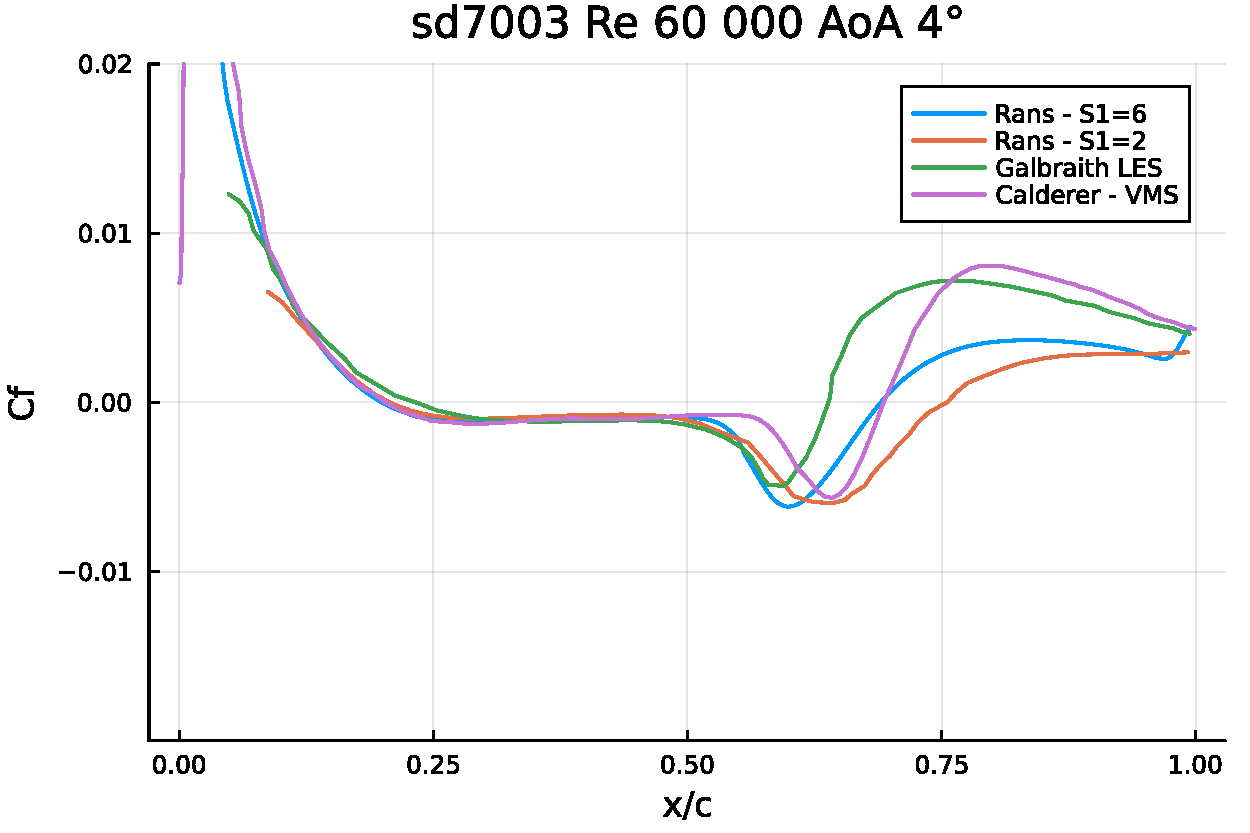
\includegraphics[width=0.65\textwidth]{ sd7003_differentmodels.pdf}
         \caption{Different model provides different results. RANs use $\gamma -Re_ \theta$ model.}
     \end{figure} 
\end{frame}




\begin{frame}{VMS linearized coupled sd7003s}
Coupled: velocity and pressure are solved at the same time.
Re $\num{60000}$ - AoA $\ang{4}$ . Initialization with velocity-ramping
\begin{figure}[h]
     \centering          
     \begin{subfigure}[h]{0.45\textwidth}
              \centering
         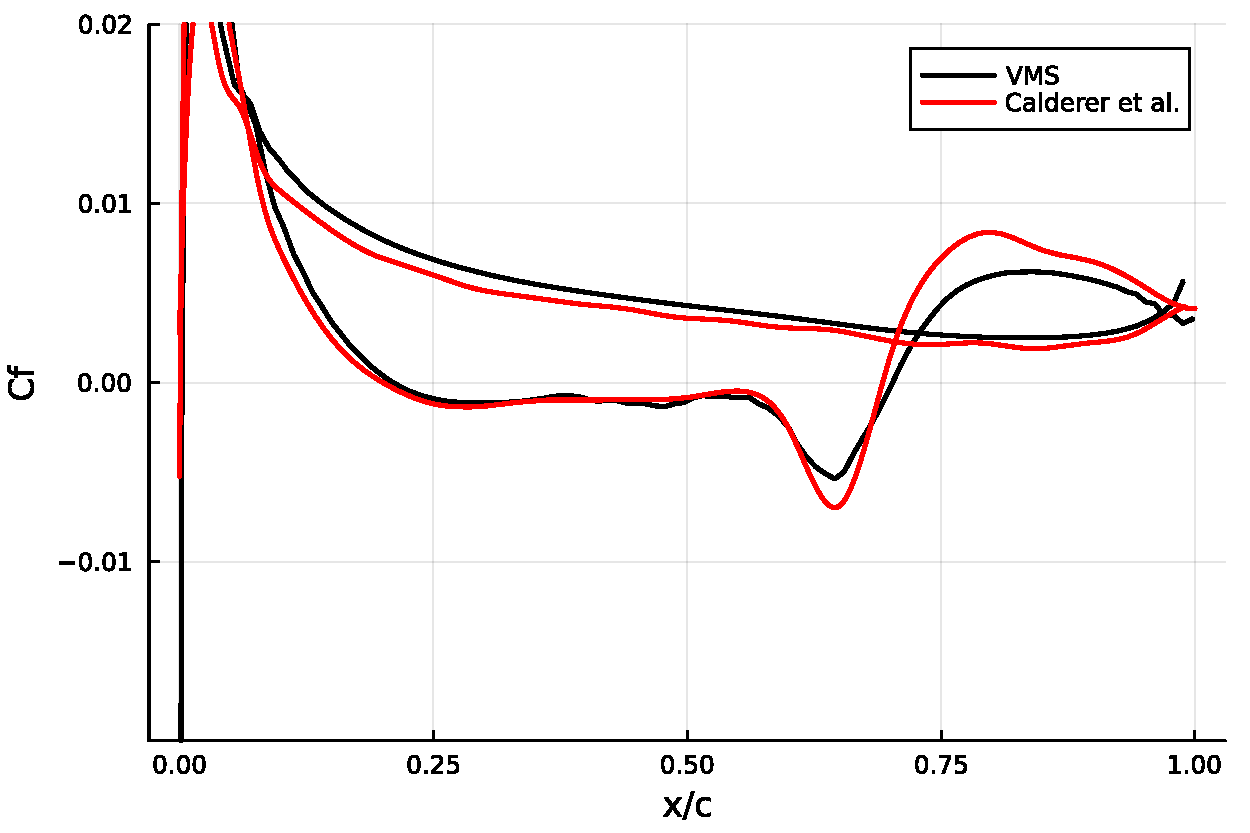
\includegraphics[width=\textwidth]{sd7003_cf.pdf}
    \end{subfigure}
          \hfill
     \begin{subfigure}[h]{0.45\textwidth}
      \centering
         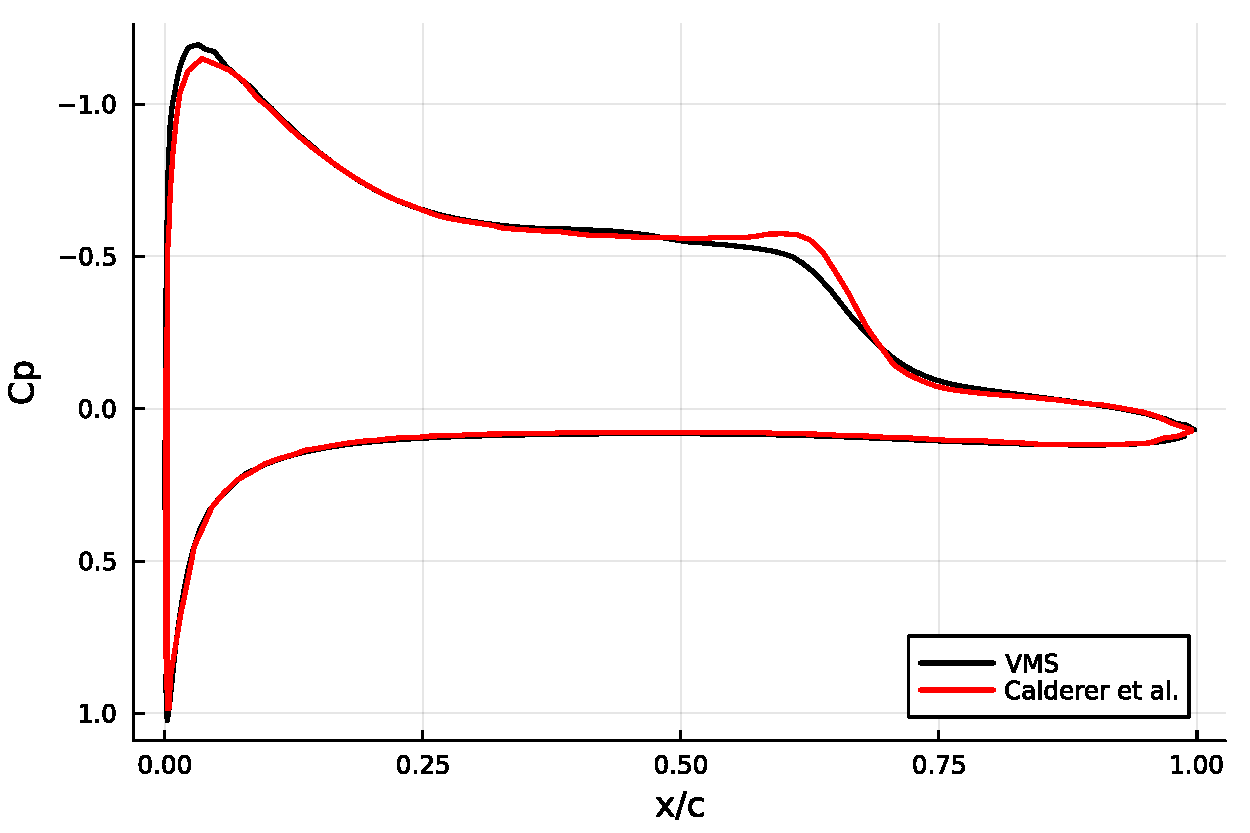
\includegraphics[width=\textwidth]{sd7003_cp.pdf}
     \end{subfigure}
\caption{Comparison with VMS literature results}
     \end{figure} 
     
\end{frame}

\begin{frame}{ VMS linearized coupled sd7003s}
\begin{figure}[h]
     \centering          
         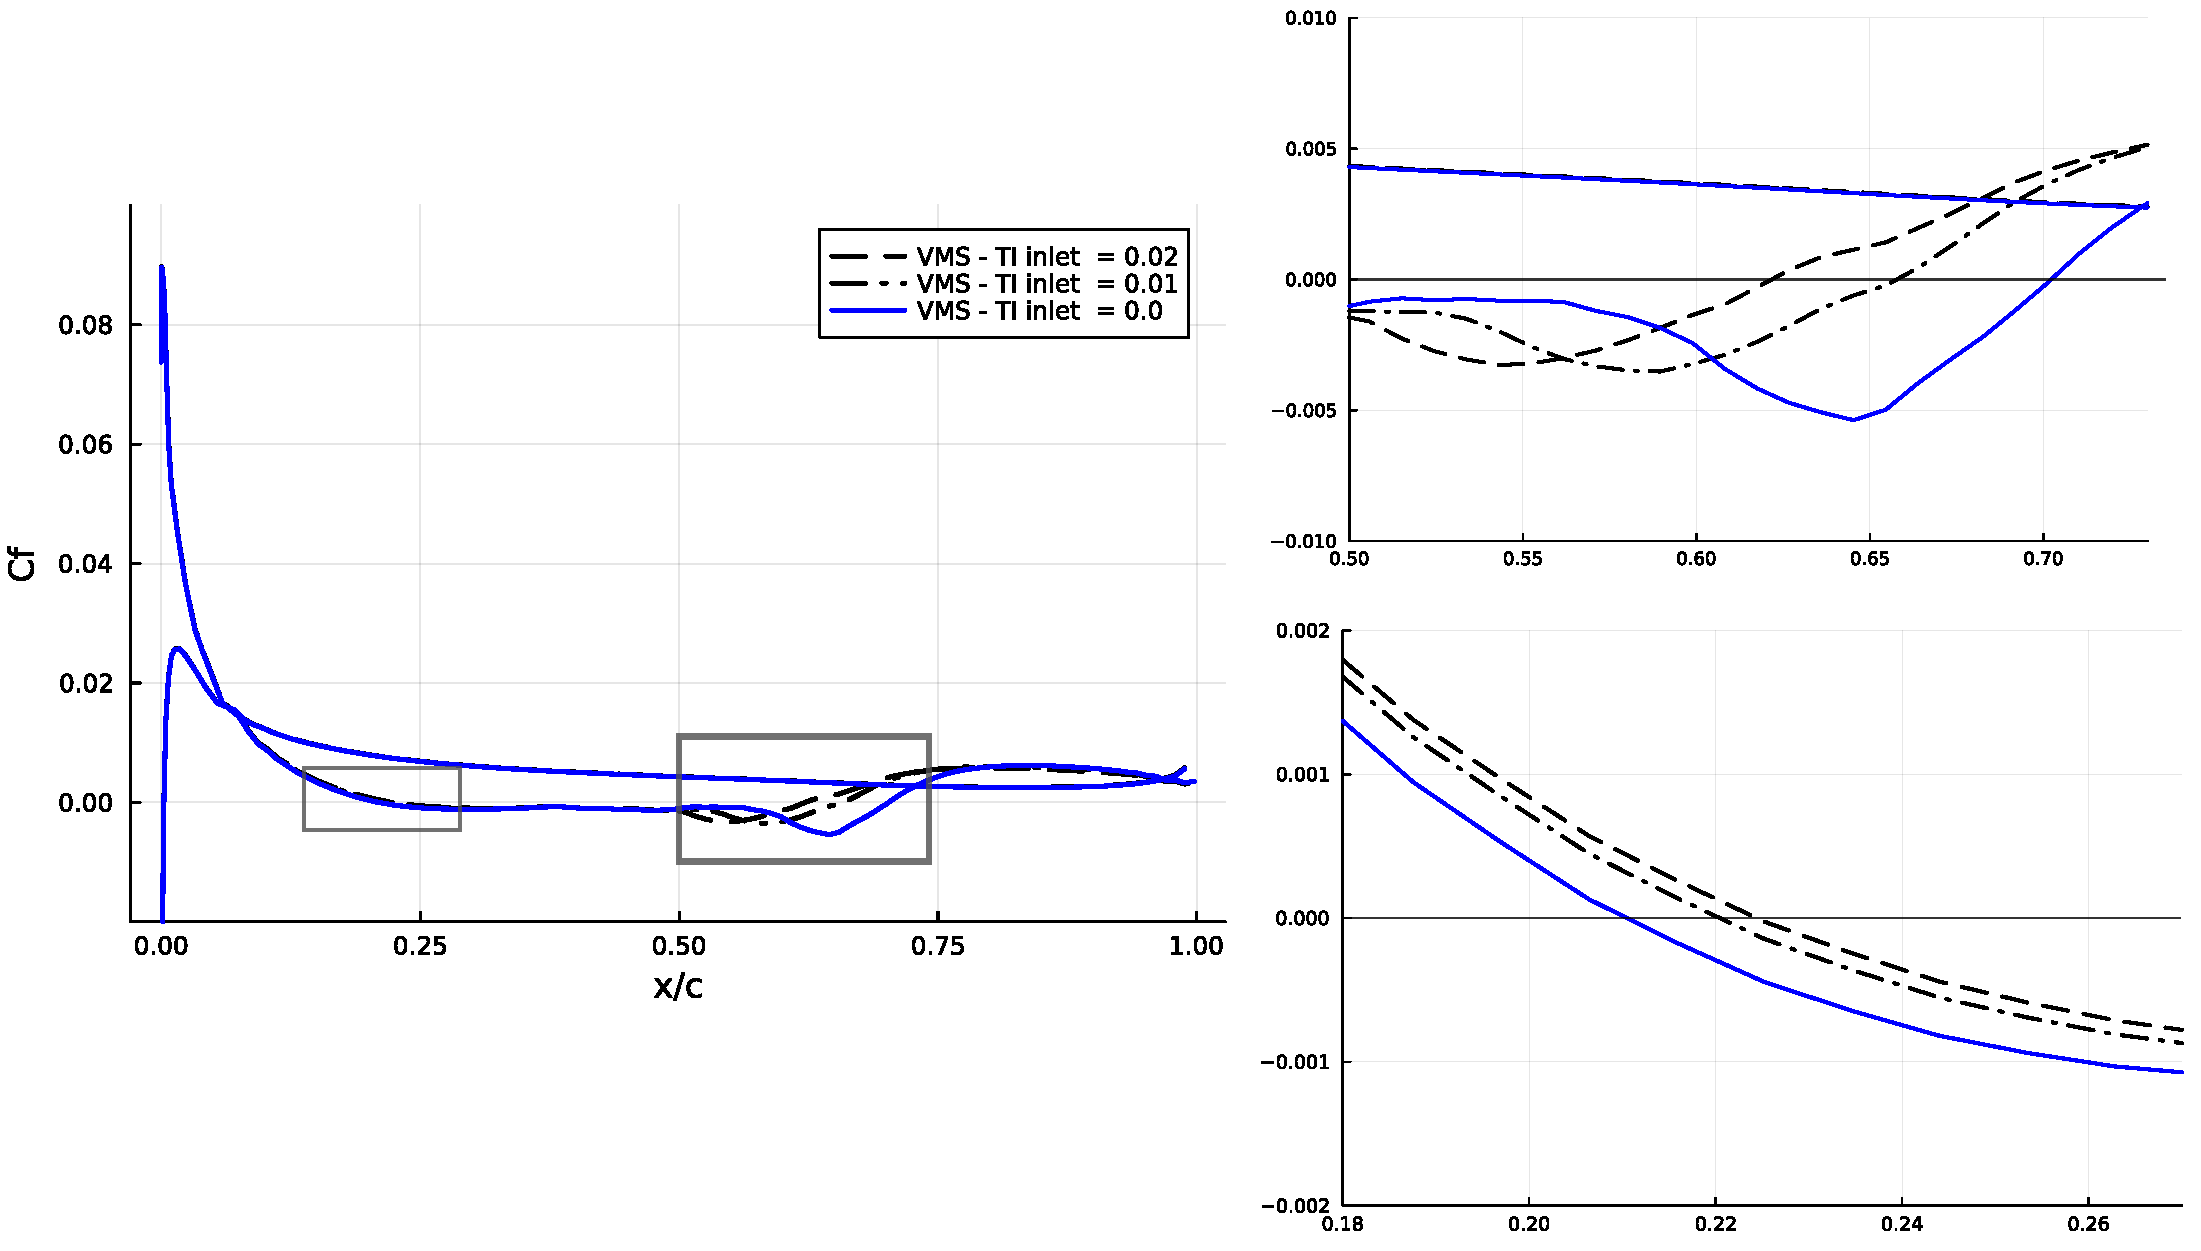
\includegraphics[width=0.8\textwidth]{SD7003_Cf_zoom.pdf}
         \caption{Bubble position function of freestream turbulence intensity}
     \end{figure} 
\end{frame}




\begin{frame}{VMS Linearized-Segregated}
Segregated: each time step pressure and velocity system are solved one after the other multiple times. It is possible to re-use the matrices and preconditioner. It is an iterative method.
\begin{figure}[h]
     \centering          
         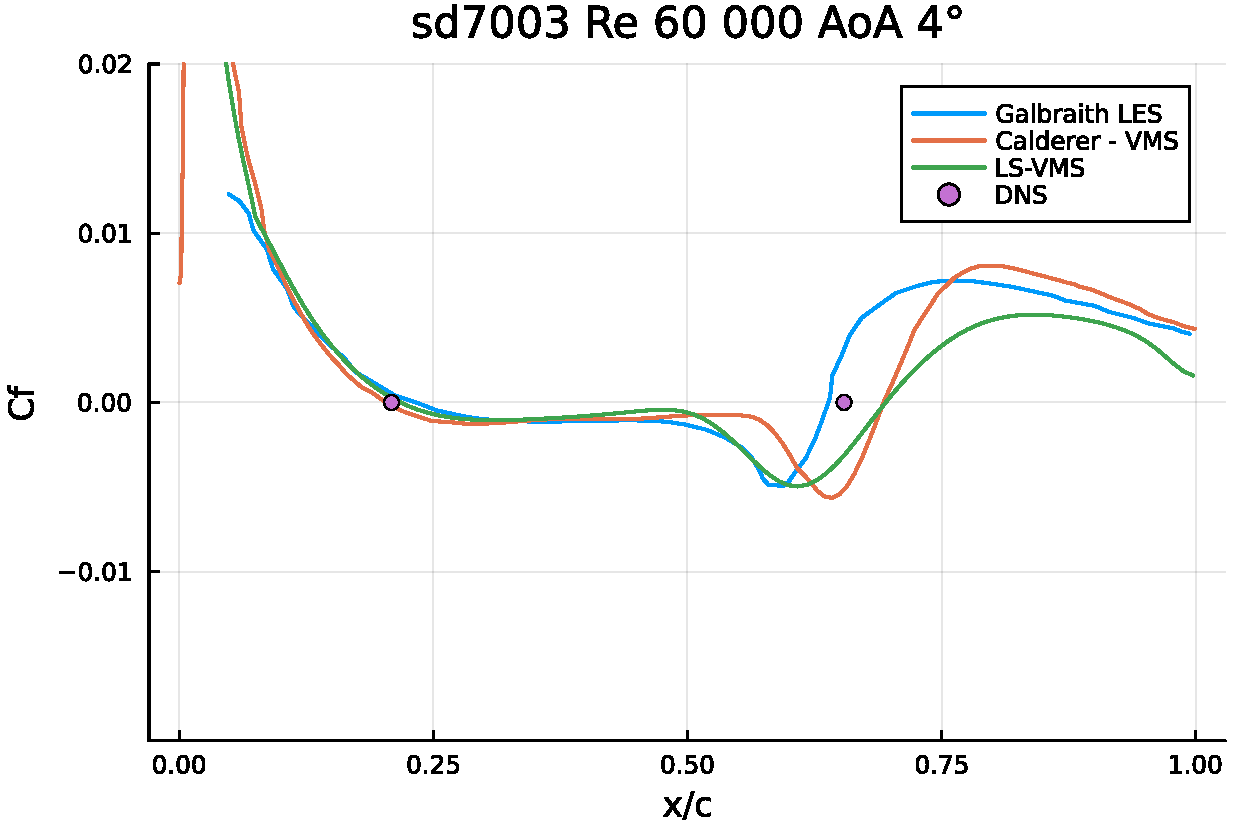
\includegraphics[width=0.65\textwidth]{ VMS7003s_comparison.pdf}
         \caption{Different model provides different results, VMS and LES}
     \end{figure} 
\end{frame}




\begin{frame}{VMS Linearized-Segregated}
PhD research aims to simulate a new airfoil.
Re $\num{250000}$ - AoA $\ang{1}$ 

\begin{figure}[h]
     \centering          
     \begin{subfigure}[h]{0.45\textwidth}
              \centering
         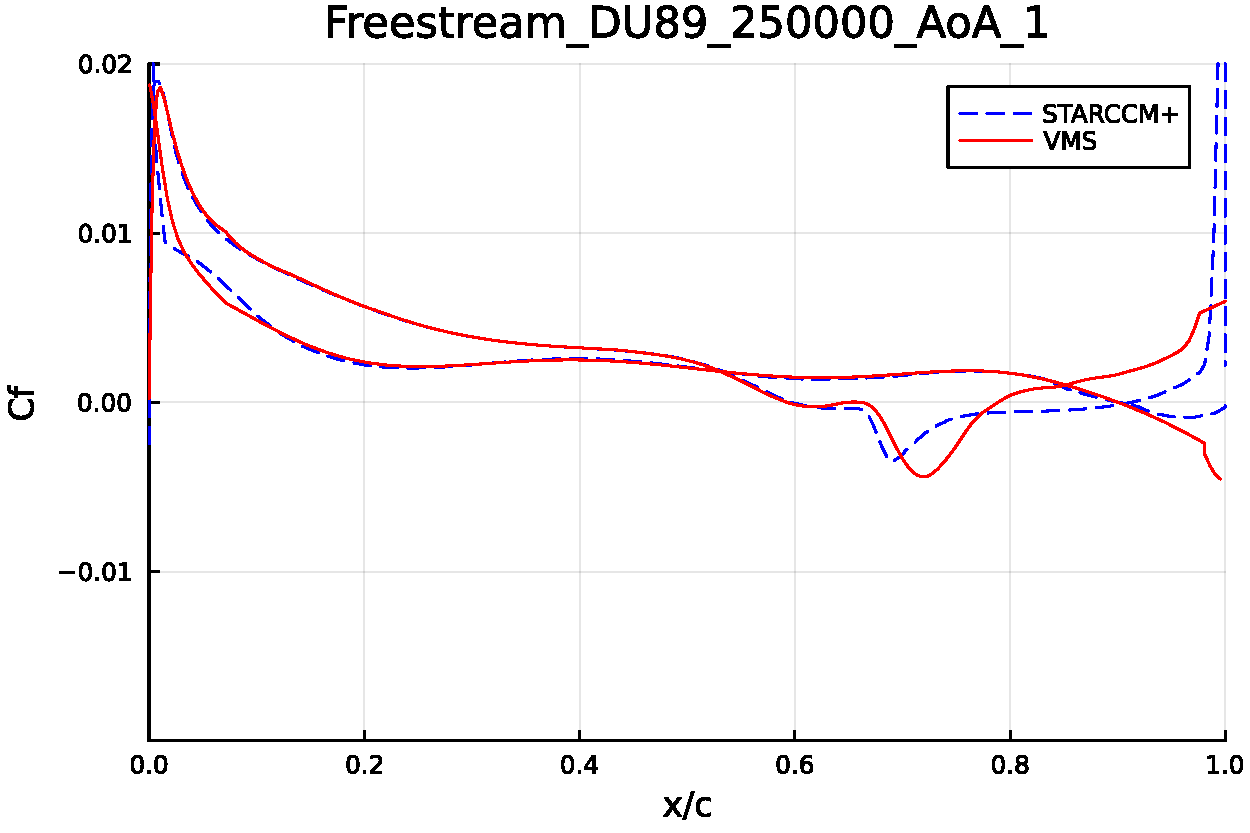
\includegraphics[width=\textwidth]{Freestream_DU89_250000_AoA_1_Cf.pdf}
    \end{subfigure}
          \hfill
     \begin{subfigure}[h]{0.45\textwidth}
      \centering
         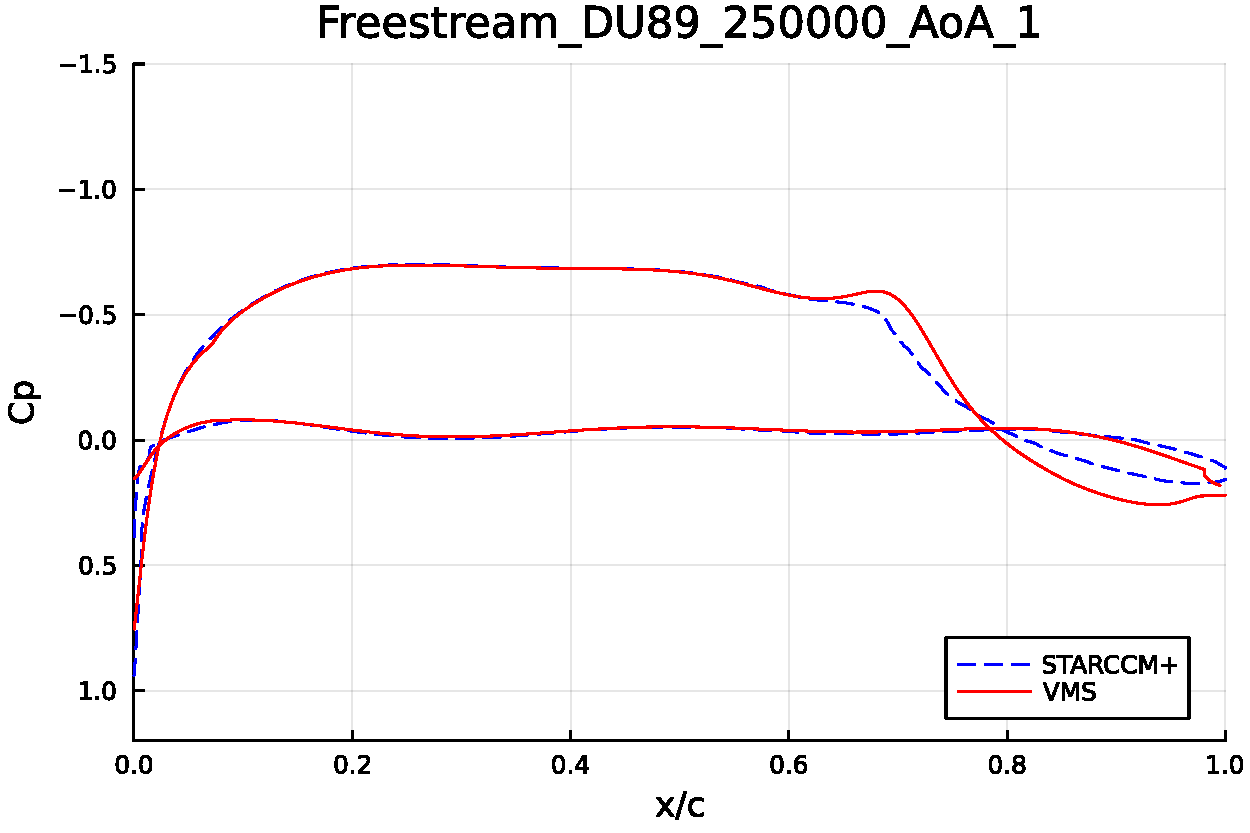
\includegraphics[width=\textwidth]{Freestream_DU89_250000_AoA_1_Cp.pdf}
     \end{subfigure}
     \end{figure} 
 \end{frame}

\begin{frame}{VMS Linearized-Segregated}
Re $\num{250000}$ - AoA $\ang{5}$ 
\begin{figure}[h]
     \centering          
     \begin{subfigure}[h]{0.45\textwidth}
              \centering
         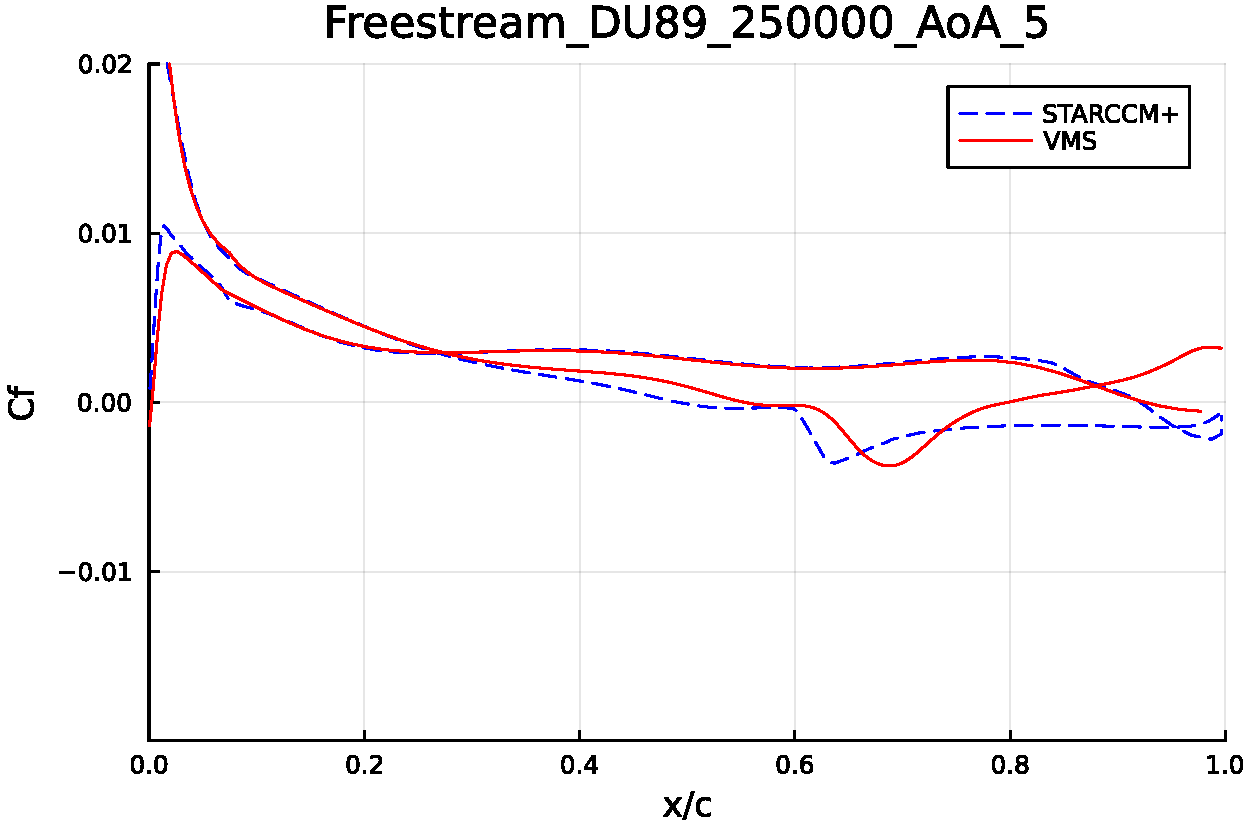
\includegraphics[width=\textwidth]{Freestream_DU89_250000_AoA_5_Cf.pdf}
    \end{subfigure}
          \hfill
     \begin{subfigure}[h]{0.45\textwidth}
      \centering
         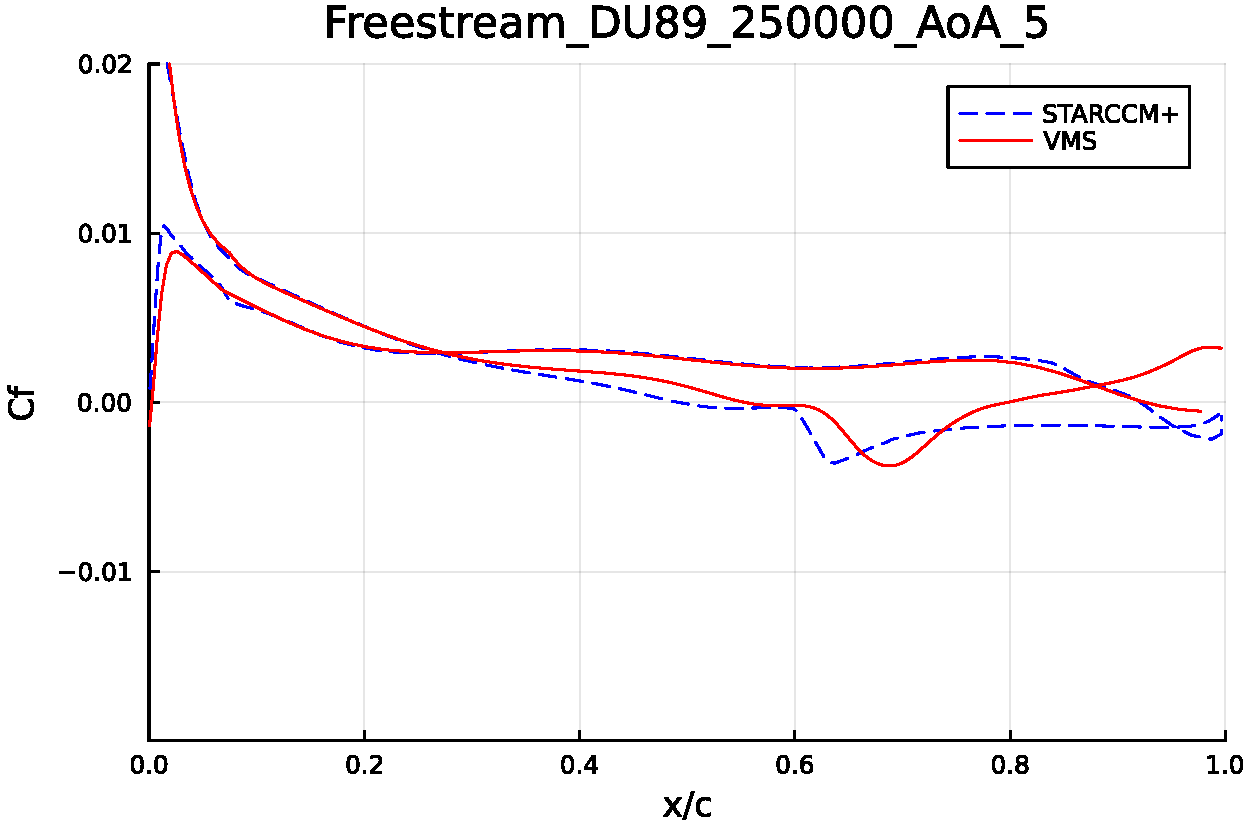
\includegraphics[width=\textwidth]{Freestream_DU89_250000_AoA_5_Cp.pdf}
     \end{subfigure}
     \end{figure} 
 \end{frame}

\begin{frame}{VMS Linearized-Segregated}
Re $\num{500000}$ - AoA $\ang{1}$ 
\begin{figure}[h]
     \centering          
     \begin{subfigure}[h]{0.45\textwidth}
              \centering
         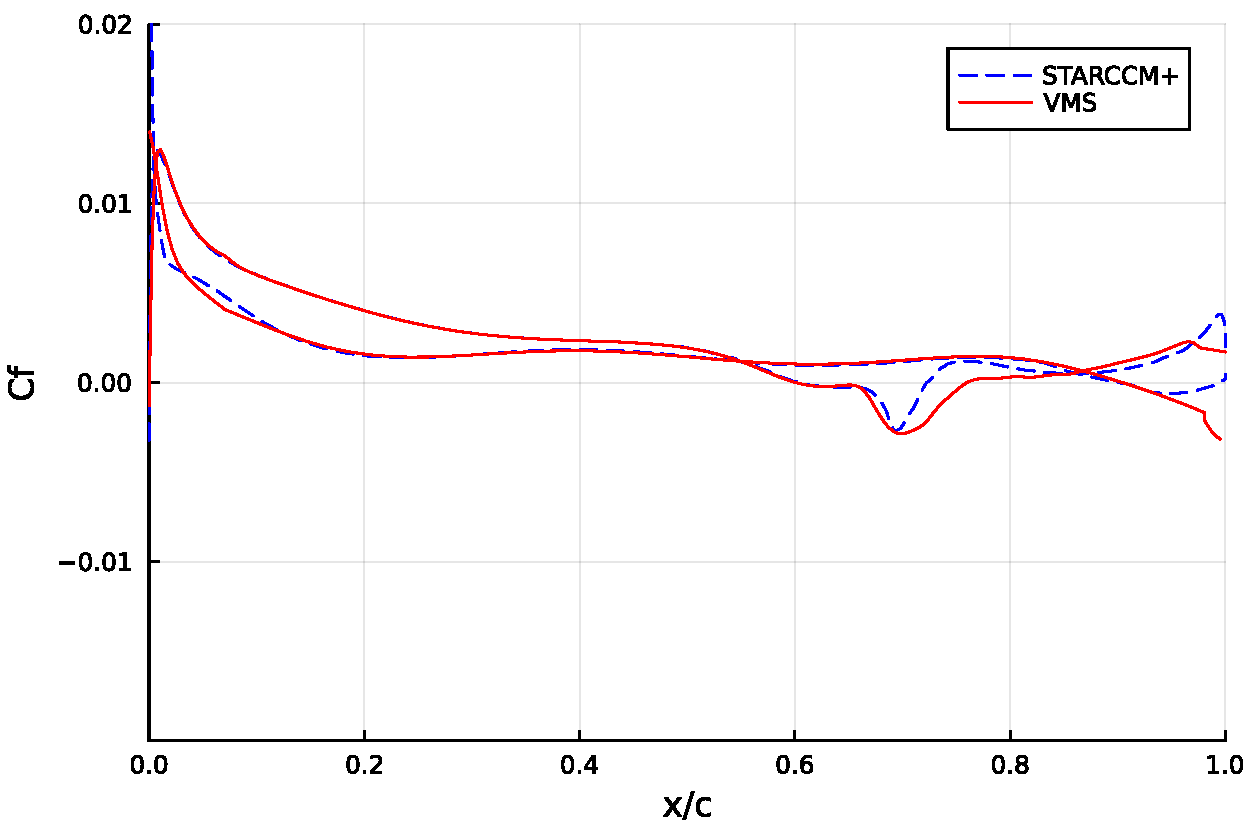
\includegraphics[width=\textwidth]{Freestream_DU89_500000_AoA_1_Cf.pdf}
    \end{subfigure}
          \hfill
     \begin{subfigure}[h]{0.45\textwidth}
      \centering
         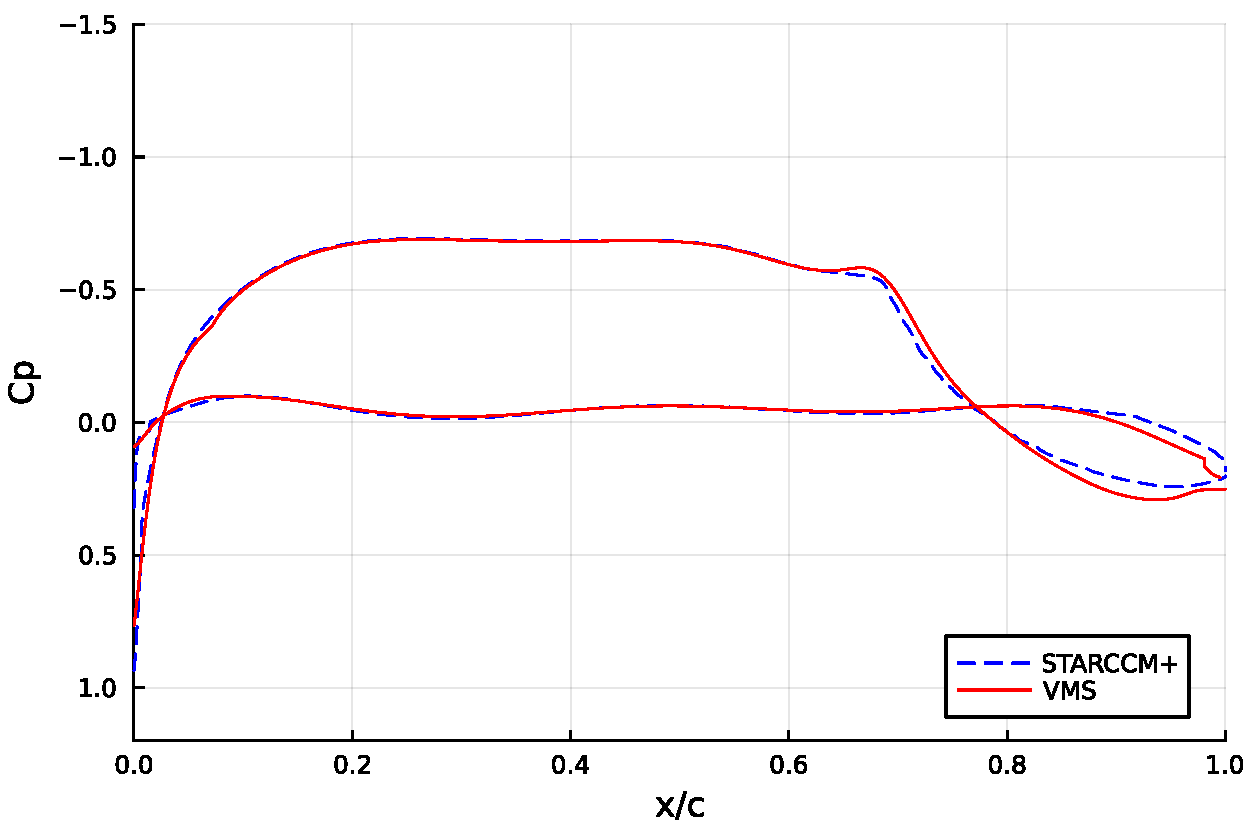
\includegraphics[width=\textwidth]{Freestream_DU89_500000_AoA_1_Cp.pdf}
     \end{subfigure}
     \end{figure} 
 \end{frame}

\begin{frame}{VMS Linearized-Segregated}
Re $\num{500000}$ - AoA $\ang{5}$ 
\begin{figure}[h]
     \centering          
     \begin{subfigure}[h]{0.45\textwidth}
              \centering
         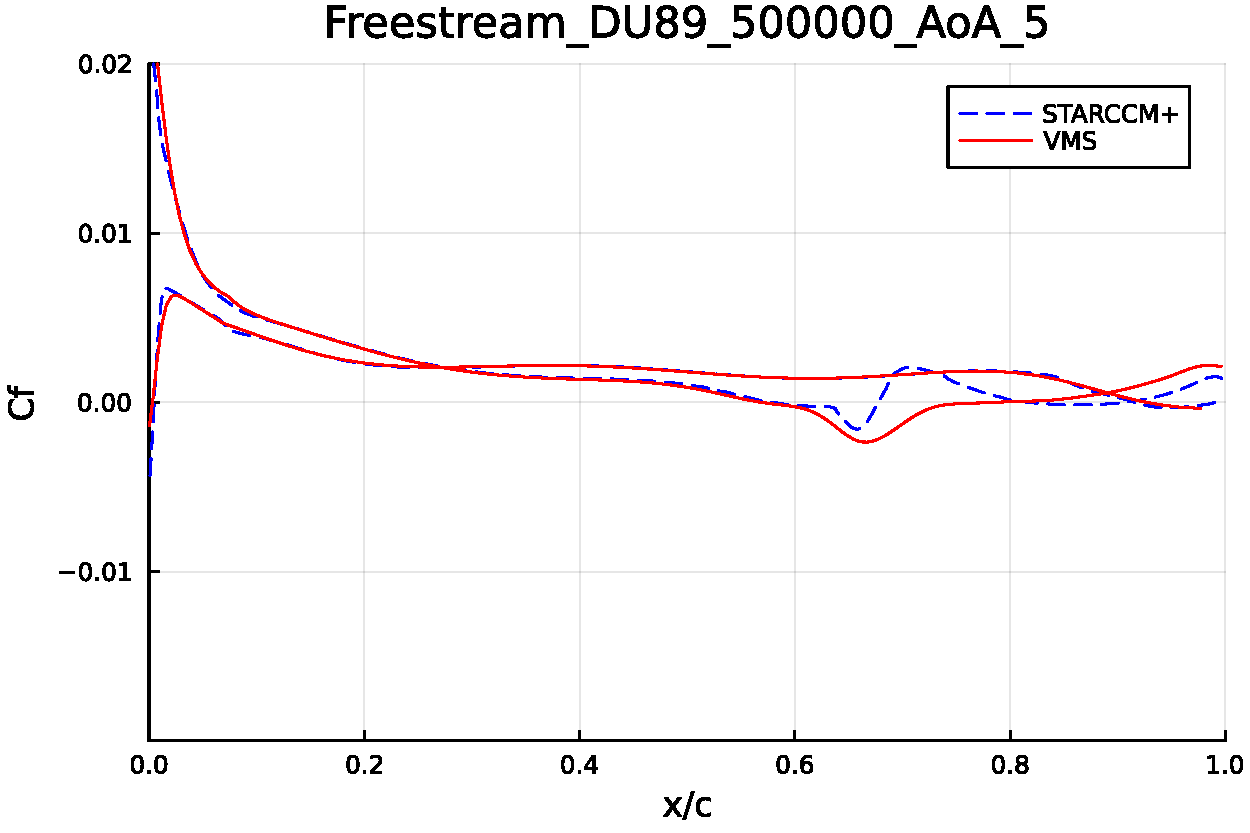
\includegraphics[width=\textwidth]{Freestream_DU89_500000_AoA_5_Cf.pdf}
    \end{subfigure}
          \hfill
     \begin{subfigure}[h]{0.45\textwidth}
      \centering
         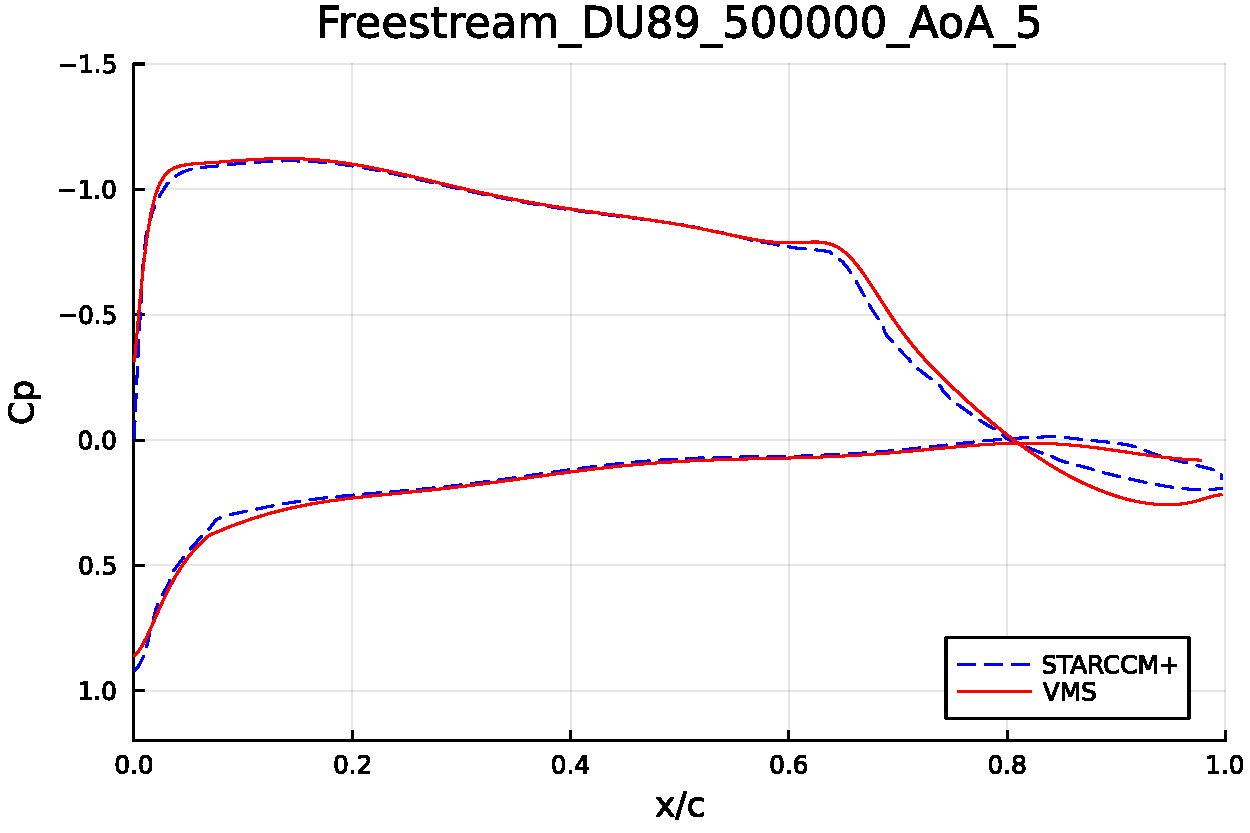
\includegraphics[width=\textwidth]{Freestream_DU89_500000_AoA_5_Cp.pdf}
     \end{subfigure}
     \end{figure} 
 \end{frame}


\begin{frame}{Mesh Sensitivity}
\begin{table}[!ht]
     \centering
     \begin{tabular}{l|llll}
         \hline
         Mesh settings & $\mathcal{C}$ & $\mathcal{M}$ & $\mathcal{F}$ & $\mathcal{SF}$ \\  \hline
         Airfoil divisions & 150 & 200 & 200 & 300 \\ 
         Z divisions & 12 & 16 & 22 & 16 \\ 
         First cell height [m] & 4.8e-6 & 2.8e-6 & 1.6e-6 & 1.6e-6 \\ 
         Number of Cells & 4.1e5 & 6.6e5 & 8.5e6 & 8.9e6 \\ \hline
         CL & 0.3539 & 0.3514 & 0.3504 & 0.3519 \\
         CD & 0.00915 & 0.00950 & 0.00929 & 0.00947 \\ 
         Separation (x/c) & 0.60 & 0.60 & 0.60 & 0.60 \\ 
     \end{tabular}
 \caption{Mesh sensitivity analysis DU89, Reynolds $\num{500000}$, Aoa $\ang{1}$}
 \label{tab:mesh-sensitivity-re500000}
 \end{table}
\end{frame}


\begin{frame}{Time Sensitivity}
     \begin{table}[!ht]
          \centering
          
              \begin{tabular}{l|llll}
                  \hline
                  Mesh & $\mathcal{C}$ & $\mathcal{C}$  & $\mathcal{M}$ & $\mathcal{M}$ \\  
                  \hline
                  Time average[s] & 10  & 20 & 10 & 20 \\  
                  CL&0.3538 & 0.3539 & 0.3516 & 0.3514	 \\
                  CD& 0.00910 &0.00915 & 0.00939& 0.00950  \\ 
                  Separation (x/c) & 0.60 & 0.60 & 0.60 & 0.60 \\ 
              \end{tabular}
              
          \caption{Time average sensitivity analysis DU89, Reynolds $\num{500000}$, Aoa $\ang{1}$}
          \label{tab:time-sensitivity-re500000}
     \end{table}

     \begin{table}[!ht]
          \centering
              \begin{tabular}{l|lll}
                  \hline
                  dt$[s]$ & $2\;10^{-3}$  & $1\;10^{-3}$ & $5\;10^{-4}$ \\  \hline
                  CL & diverged & 0.3514  & 0.3511 \\
                  CD & diverged & 0.00950 & 0.00911  \\ 
                  Separation (x/c) & diverged & 0.60 & 0.60 \\ 
              \end{tabular}
              
          \caption{Time sensitivity analysis DU89, Reynolds $\num{500000}$, Aoa $\ang{1}$}
          \label{tab:time-sensitivity-re500000}
          \end{table}
\end{frame}


\begin{frame}{VMS Linearized-Segregated}
VMS airfoil in wind tunnel
     \begin{figure}[h]
          \centering          
              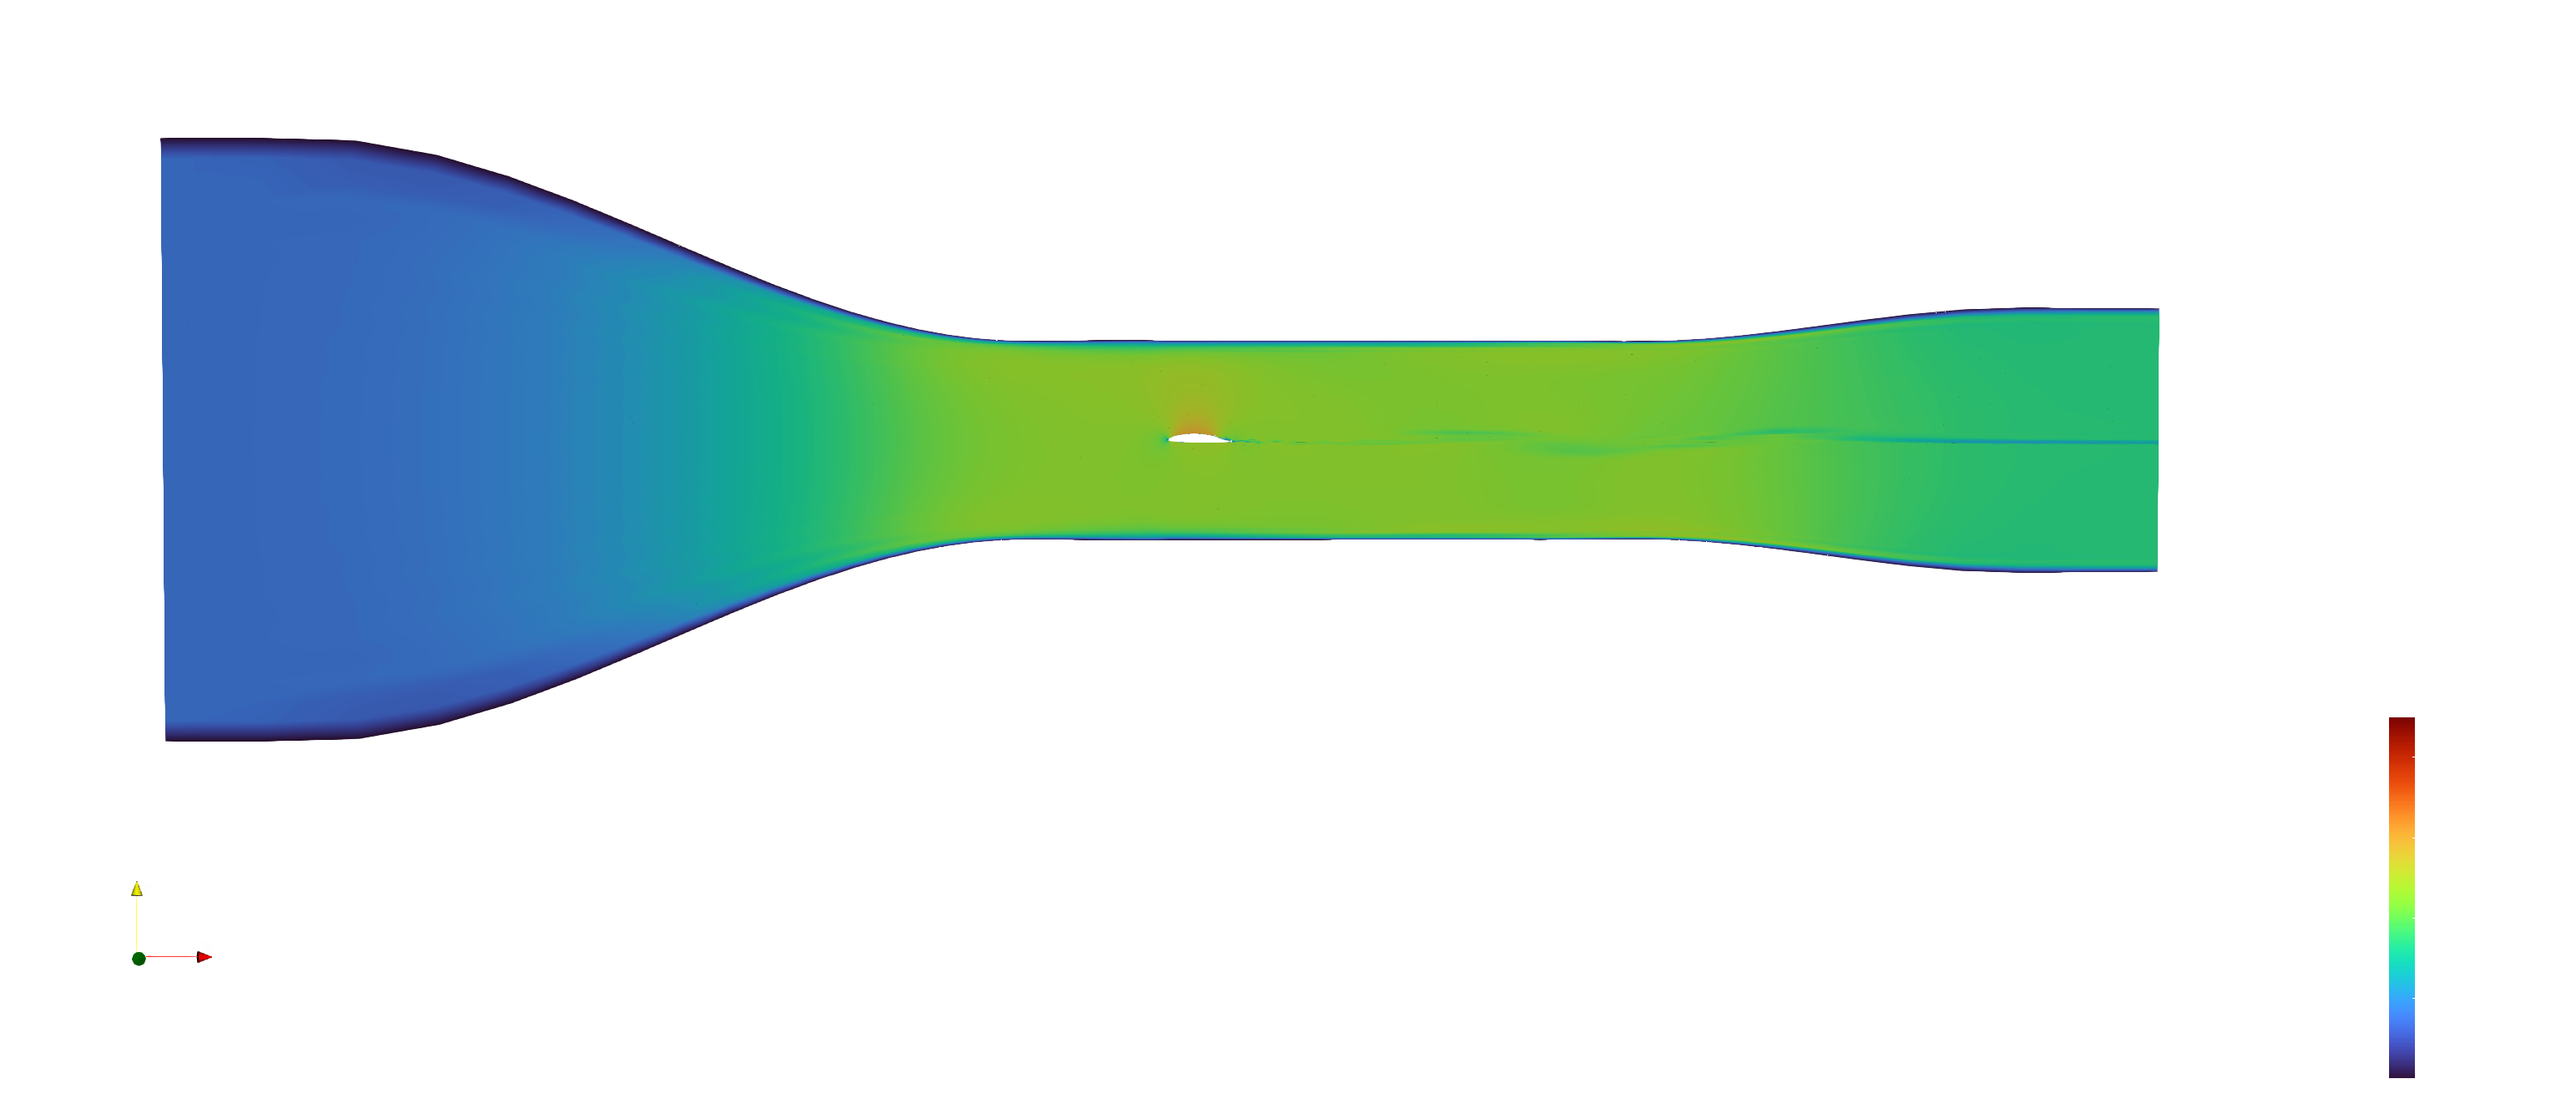
\includegraphics[width=0.65\textwidth]{DU89_WT_v.png}
              \caption{3D VMS Wind Tunnel simulation with DU89}
          \end{figure} 
\end{frame}